\section{Использование системных служебных функций DNS}

Для поддержания работы сети Интернет были введены служебные протоколы, к которым относится DNS. Данный протокол позволяет по доменному имени получить IP адрес сервера, отвечающего за работу данного сайта. Для этого требуется выполнить несколько запросов к DNS серверам. Они начинаются с анализа файла host, а затем происходит обращение к серверу провайдера, корневым серверам, серверам зоны\dots Поскольку количество запросов отправляемые к серверам велико, то для обеспечения быстродействия работы через интернет системы защиты информации часто не проверяют сервера, на которые передают запрос, на недостоверность. Данную ситуацию сильно усугубляет существование DNS серверов, способные выполнять рекурсивные запросы. 

Проанализировав данный протокол возникло предположение, что возможно построить с помощью него скрытый канал передачи информации, скомпрометировав DNS нескольких доменов и используя их субдомены как средство передачи данных.

При реализации было учтено, что злоумышленник может использовать не только скомпрометированные сервера, но и свои с установленными на них соответствующих программ. Поэтому был создан сервер с установленным на нем программного обеспечением Bind, позволяющим организовать DNS сервер, который был настроен так, что все запросы, адресованные к нему, обрабатывались и сохранялись. Также был зарегистрирован домен proxy.myprogram.us, который был привязан к созданному серверу. Разработано программное обеспечение, которое всю информацию, передаваемую через DNS канал, шифровало методом сдвига, разбивало на порции по 50 символов и полученные строки интерпретировало как субдомены домена proxy.myprogram.us и выполняло DNS запрос. Таким образом был получен канал передачи информации через протокол системного уровня --- DNS.

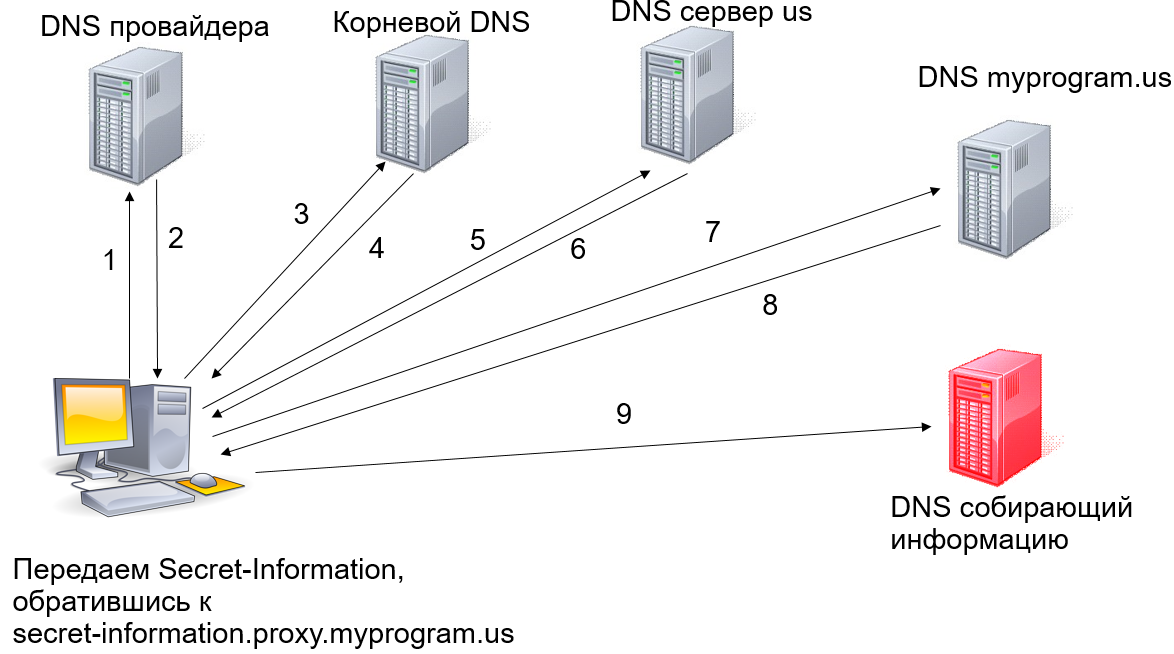
\includegraphics[width=1\linewidth]{3--dns.png}

Тестирование данного канала с работающей DLP системой было успешным. Comodo Firefall не смог обнаружить этот скрытый канал и данные были переданы на удаленный сервер.
